\chap{关于\LaTeX{}}
\label{chap_tools}  % 供后文引用

\sect{\LaTeX{}简介}
\LaTeX{}(发音<<Lah-tech>>或<<Lay-tech>>)是用于高质量排版的文本准备系统,它致力于实现内容与格式的分离,使用者只需专注于自己撰写的内容而不用过多地关注文本格式。\LaTeX{} 可以用于排版各种类型的文献,包括但不限于期刊文章、技术报告、书籍和幻灯片。\LaTeX{} 的更多特点参见 \href{https://www.latex-project.org/about/}{latex-project.org/about/} 。

\sect{\LaTeX{}安装}
\subsect{安装 \TeX{} Live}

本小节主要参考 \href{https://zhuanlan.zhihu.com/p/362201376}{zhuanlan.zhihu.com/p/362201376} 撰写。

\TeX{} Live 是一个发行版封装,里面包含了编译器,编辑器和各种宏包。安装 \TeX{} Live 后你就可以开始使用 \LaTeX{} 了。

(1)从 \href{https://mirror.ctan.org/systems/texlive/Images/}{mirror.ctan.org/systems/texlive/Images/} 下载最新的 texlive.iso 镜像文件,目前的版本是20220321。约 4.3 GB ,耗时 10+ 分钟 。

\begin{figure}[H]  % 禁止浮动
  \centering  % 表格居中
  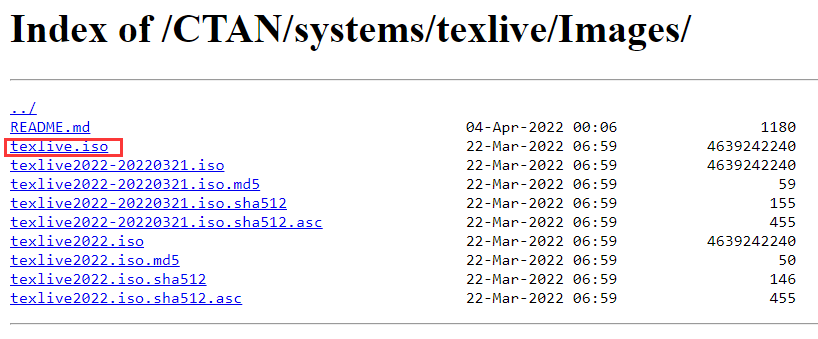
\includegraphics[scale=.5]{figure/texliveImages.png}  % 选项代表缩小到原图的 0.5 倍。

  {\zihao{-5} 图中的三个iso文件都没有区别。}  % 图注
  \caption{texlive 镜像文件}  % 图题
  \label{fig:tools:texliveImages}  % 定义标签,方便引用该图
\end{figure}

(2)下载完成后,右键>装载。在打开的文件夹(新增的DVD驱动器)中找到文件 install-tl-windows.bat ,然后右键>以管理员身份运行。

\begin{figure}[H]  % 禁止浮动
  \centering  % 表格居中
  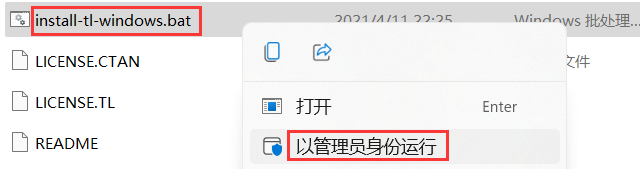
\includegraphics[scale=.5]{figure/installbat.png}  % 选项代表缩小到原图的 0.5 倍。
  \caption{运行安装程序}  % 图题
  \label{fig:tools:bat}  % 定义标签,方便引用该图
\end{figure}

(3)运行后来到 texlive 安装界面。默认安装在 C 盘,位置可修改( texlive 发行版约有 7.3 GB ,因此不建议装在 C 盘)。图 \ref{fig:tools:texliveInstaller} 所示安装界面选择了 D:/Program Files/texlive/2022 文件夹。最后点击安装,等待一两小时即可安装完成。

\begin{figure}[H]  % 禁止浮动
  \centering  % 表格居中
  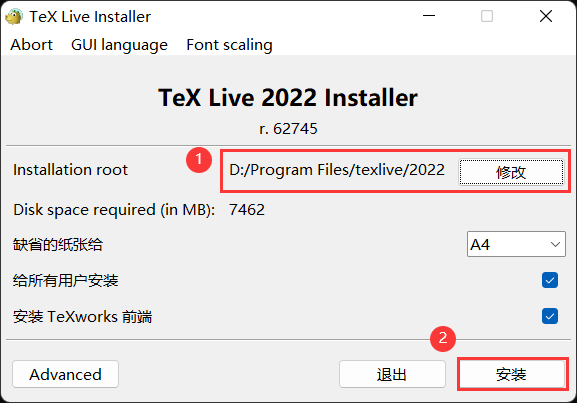
\includegraphics[scale=.5]{figure/texliveInstaller.png}  % 选项代表缩小到原图的 0.5 倍。

  {\zihao{-5} 点击左下角的 Advanced 选项可以进行更多配置,不过新手暂时不用了解。}  % 图注
  \caption{修改位置并安装}  % 图题
  \label{fig:tools:texliveInstaller}  % 定义标签,方便引用该图
\end{figure}

(4)安装完成后弹出新增的DVD驱动器。将之前下载的 iso镜像文件删除(回收站的iso文件也可以清除)。这一步是为了释放存储空间,毕竟镜像文件有 4 个 G !

\sect{\LaTeX{}编辑器的选择与配置}

\subsect{\TeX{works}配置}
安装 \TeX{} Live 发行版时会默认安装 \TeX{works} 编辑器。

可以根据自身需要在“编辑>首选项”中对 \TeX{works} 进行配置。本节将简单介绍一些方便本模板使用的基本配置。

(1)开启行号选项。进入“编辑>首选项>编辑器”,将行号前的 $\square$ 勾选。

\begin{figure}[H]  % 禁止浮动
  \centering  % 表格居中
  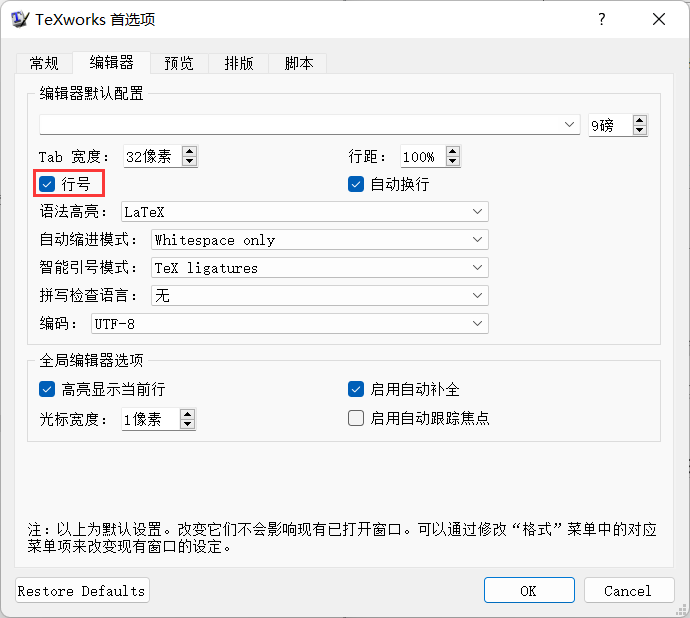
\includegraphics[scale=.45]{figure/texworkln.png}  % 选项代表缩小到原图的 0.5 倍。
  \caption{勾选行号}  % 图题
  \label{fig:tools:texworkln}  % 定义标签,方便引用该图
\end{figure}

(2)将常用处理工具的位置前置。进入“编辑>首选项>排版”,将 XeLaTeX 与 Biber 移到最前,并将默认处理工具设为 XeLaTeX 。

\begin{figure}[H]  % 禁止浮动
  \centering  % 表格居中
  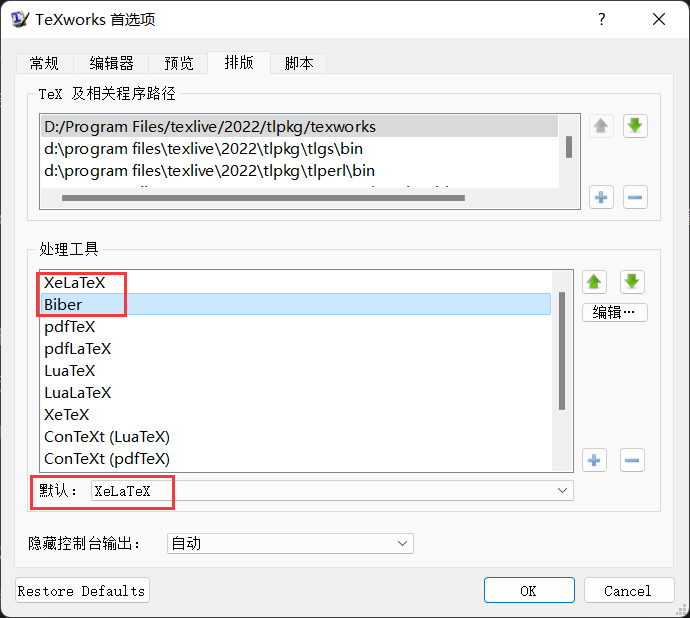
\includegraphics[scale=.45]{figure/texworkpt.png}  % 选项代表缩小到原图的 0.5 倍。
  \caption{设置默认处理工具}  % 图题
  \label{fig:tools:texworkpt}  % 定义标签,方便引用该图
\end{figure}

配置完成后记得点击 “OK” 按钮,如果配置没有生效,重新打开 \TeX{works} 即可。


\subsect{\TeX{studio}配置}
请自行了解并下载 \TeX{studio}。

\subsect{vscode配置}
请参考 \href{https://zhuanlan.zhihu.com/p/166523064}{vscode配置LaTeX} ,或者自行搜索其他资料进行配置。